\documentclass{article}

\usepackage{fancyhdr}
\usepackage{extramarks}
\usepackage{amsmath}
\usepackage{amsthm}
\usepackage{amsfonts}
\usepackage{tikz}
\usepackage[plain]{algorithm}
\usepackage{algpseudocode}

\usetikzlibrary{automata,positioning}

%
% Basic Document Settings
%

\topmargin=-0.45in
\evensidemargin=0in
\oddsidemargin=0in
\textwidth=6.5in
\textheight=9.0in
\headsep=0.25in

\linespread{1.1}

\pagestyle{fancy}
\rhead{\firstxmark}
\lfoot{\lastxmark}
\cfoot{\thepage}

\renewcommand\headrulewidth{0.4pt}
\renewcommand\footrulewidth{0.4pt}

\setlength\parindent{0pt}

%
% Create Problem Sections
%

\newcommand{\enterProblemHeader}[1]{
    \nobreak\extramarks{}{Problem \arabic{#1} continued on next page\ldots}\nobreak{}
    \nobreak\extramarks{Problem \arabic{#1} (continued)}{Problem \arabic{#1} continued on next page\ldots}\nobreak{}
}

\newcommand{\exitProblemHeader}[1]{
    \nobreak\extramarks{Problem \arabic{#1} (continued)}{Problem \arabic{#1} continued on next page\ldots}\nobreak{}
    \stepcounter{#1}
    \nobreak\extramarks{Problem \arabic{#1}}{}\nobreak{}
}

\setcounter{secnumdepth}{0}
\newcounter{partCounter}
\newcounter{homeworkProblemCounter}
\setcounter{homeworkProblemCounter}{0}
\nobreak\extramarks{Problem \arabic{homeworkProblemCounter}}{}\nobreak{}

%
% Homework Problem Environment
%
% This environment takes an optional argument. When given, it will adjust the
% problem counter. This is useful for when the problems given for your
% assignment aren't sequential. See the last 3 problems of this template for an
% example.
%
\newenvironment{homeworkProblem}[1][-1]{
    \ifnum#1>0
        \setcounter{homeworkProblemCounter}{#1}
    \fi
    \section{Problem \arabic{homeworkProblemCounter}}
    \setcounter{partCounter}{1}
    \enterProblemHeader{homeworkProblemCounter}
}{
    \exitProblemHeader{homeworkProblemCounter}
}



%
% Homework Details
%   - Title
%   - Due date
%   - Class
%   - Section/Time
%   - Instructor
%   - Author
%

\newcommand{\hmwkTitle}{Final Project}
\newcommand{\hmwkName}{Digit/Face Recognition}
\newcommand{\hmwkDate}{May 1, 2023}
\newcommand{\hmwkClass}{CS 440: Introduction to Artificial Intelligence}
\newcommand{\hmwkClassInstructor}{Professor Abdelsam Boularias}


%
% Title Page
%

\title{
    \vspace{2in}
    \textmd{\textbf{\hmwkClass}}\\
    \textmd{\hmwkTitle\ \hmwkName}\\
    \vspace{0.1in}\small{\hmwkDate}\\
    \vspace{0.1in}\large{\textit{\hmwkClassInstructor}}
    \vspace{3in}
}

\author{
    \textbf{Jay Patwardhan} {RUID}\\ 
    \textbf{Alan Wu} {208000574}\\ 
    \textbf{Neel Shejwalkar} {RUID}
}
\date{}

\renewcommand{\part}[1]{\textbf{\large Part \Alph{partCounter}}\stepcounter{partCounter}\\}

%
% Various Helper Commands
%

% Useful for algorithms
\newcommand{\alg}[1]{\textsc{\bfseries \footnotesize #1}}

% For derivatives
\newcommand{\deriv}[1]{\frac{\mathrm{d}}{\mathrm{d}x} (#1)}

% For partial derivatives
\newcommand{\pderiv}[2]{\frac{\partial}{\partial #1} (#2)}

% Integral dx
\newcommand{\dx}{\mathrm{d}x}

% Alias for the Solution section header
\newcommand{\bruh}{\textbf{\large Solution}}
\newtheorem*{solution*}{Solution}
\newenvironment{solution}{\begin{solution*}}{{\finishline} \end{solution*}}


% Probability commands: Expectation, Variance, Covariance, Bias
\newcommand{\E}{\mathrm{E}}
\newcommand{\Var}{\mathrm{Var}}
\newcommand{\Cov}{\mathrm{Cov}}
\newcommand{\Bias}{\mathrm{Bias}}

\begin{document}

\maketitle

\pagebreak

%Part 0%
\begin{homeworkProblem}
    \textbf{\large Constructing Features and Algorithms}\\\\
    Our features were each pixel: they have a status of 1 or 0 depending on whether they are black or white. The 3 algorithms are the 3 on the Berkeley website: Naive Bayes, Perceptron, and MIRA.

    Naive Bayes uses Bayes formula under the independence of feature assumption to compute probabilities, it's a straightforward algorithm, but the bookkeeping is a little tedious. We estimate parameters using the training data, and apply a smoothing constant k to reduce an overfitting concern. We find the best model over a grid of potential k values by testing each one. Finally, we compute log probabilities since multiplying probabilities results in underflow, but the monotonicity and injectivity of the logarithm function grants us that our conversion remains faithful and doesn't mess up the probabilities.
    \\\\
    Perceptron is a single layered neural network which utilizes online learning, so it takes in each sample at a time, and computes a guess, compares it to the actual label, and tweaks the weights for each label accordingly to make the correct label more likely to be the output of the prediction function. We run multiple (3) iterations of this to make sure that everything is properly tuned and trained, but we don't run it too many times to make sure that we don't overtrain on our training data. 
    \\\\
    MIRA is an extension of the perceptron, where instead of updating weights only by the vector of features, we attach a nonnegative scalar constant to the features and update by this multiplication of $\tau * f$. This scalar is chosen such that it minimizes the sum of dot products of each estimated label minus the actual label, attaching a sense of Euclidean distance metric to the space in order to find the closest possible reflection of the actual outcome. Without dealing with the technical aspects of actually minimizing this function, this comes down to selecting a minimum of some constant C, chosen to attach a maximum value of our scalar, and another value determined by taking the vector distance of the labels, multiplying by the feature function, adding 1, and dividing by the dot product of the features to keep our values from getting too large if our feature vector contains big values, in an almost normalization measure (except we miss the square root here). 
    When implementing MIRA, we test multiple values of our constants C to determine which gives us the best model for our training data, and of course we keep the multiple iteration rounds to compute and tweak our labels from the perceptron model.

\end{homeworkProblem}

\pagebreak

%Part 1%
\begin{homeworkProblem}
    \textbf{\large Naive Bayes}\\\\
    We show plots and results for Naive Bayes on faces. The digits case is close to identical, so in order to avoid redundancy we attach only the faces plots to show our results. One thing to note about the digits plots are that since the number of samples are so large, they become uniform very quickly, even from the beginning for certain tests like accuracy; even though their performance does get better with more samples, the distinction isn't as striking as the faces plots, since we only work with a maximum of 450 faces versus 5000 digits. 
    Attached are plots of the time it took to train Naive Bayes against the number of samples used to train, the mean of each iteration (10 percent, 20 percent,...,100 percent samples) against the number of samples, and finally the standard deviation of each iteration against the number of samples. Note that all samples were taken randomly from the whole.
    \\\\
    {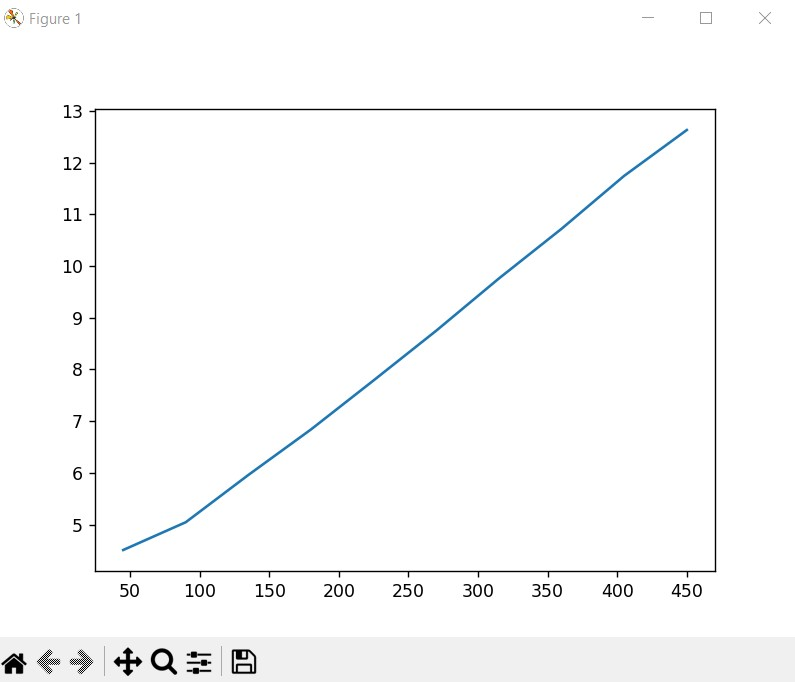
\includegraphics[width=0.75\textwidth]{faces_time.jpg}}
    \\\\
    {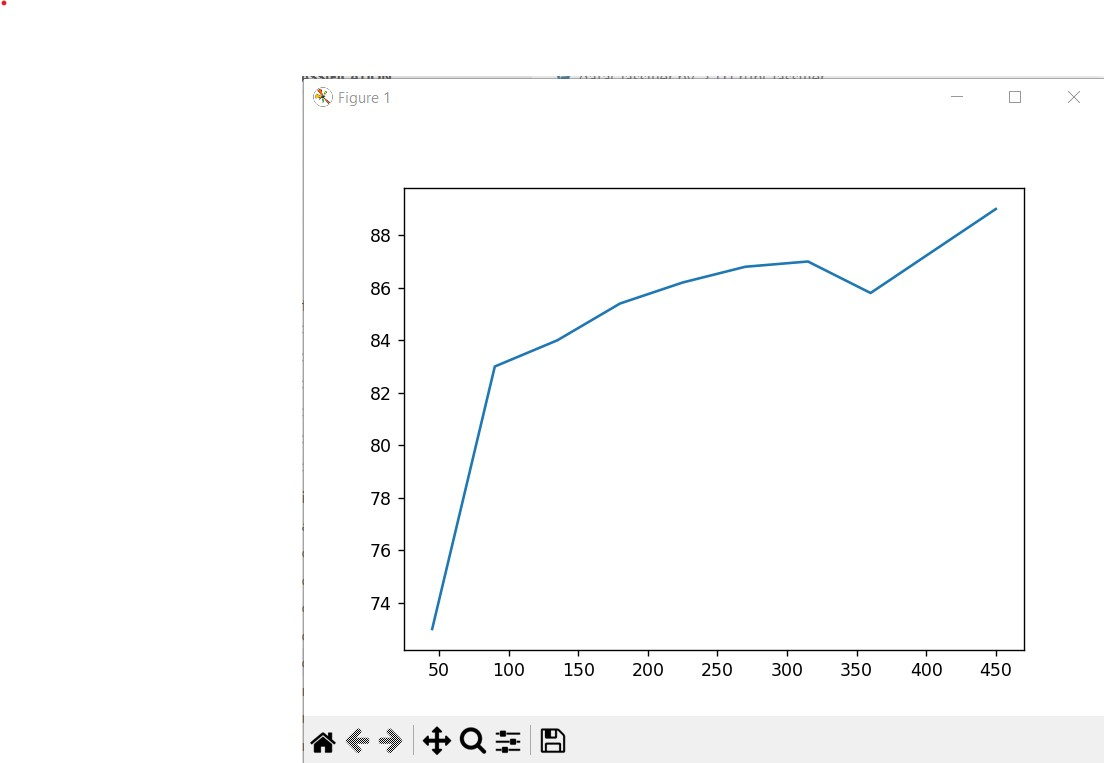
\includegraphics[width=0.75\textwidth]{faces_mean.jpg}}
    \\\\
    {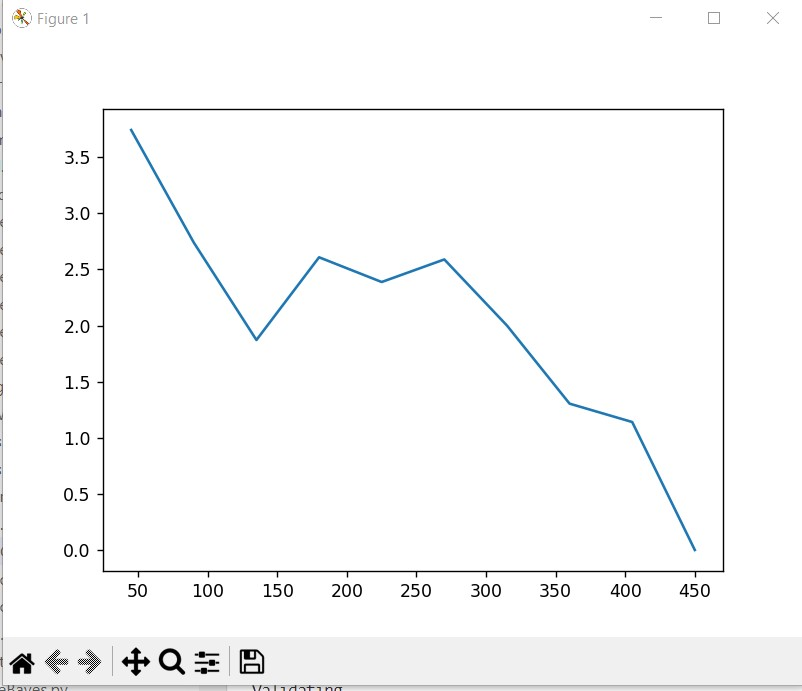
\includegraphics[width=0.75\textwidth]{faces_std.jpg}}
    \\\\

    It is clear to see as well that the mean accuracy increases with more samples and the standard deviation decreases dramatically, so the estimates get increasingly precise.
   
\end{homeworkProblem}

\pagebreak

%Part 2%
\begin{homeworkProblem}
    \textbf{\large Perceptron}\\\\
    Same as the Naive Bayes case, we show our results for faces, the digits plots have an identical discussion as the one we did for Naive Bayes.
    In the same order as above, we have the plots: time vs samples, mean vs samples, and std vs samples:
    \\\\
    {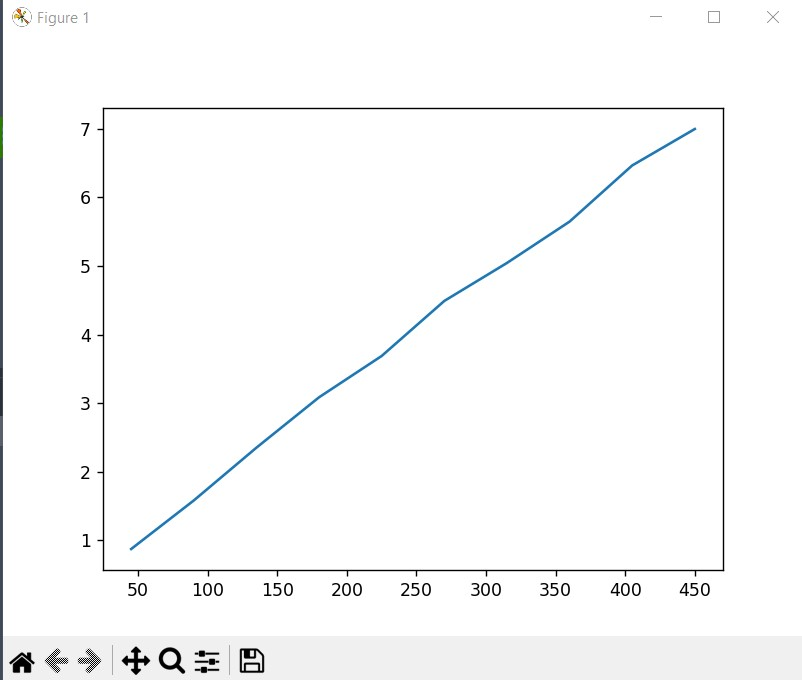
\includegraphics[width=0.75\textwidth]{perceptron_time.jpg}}
    \\\\
    {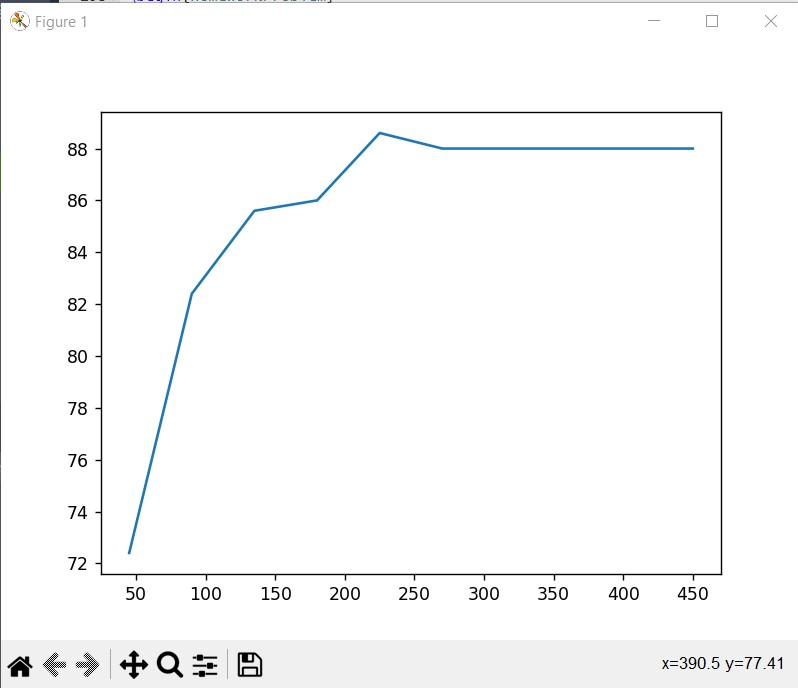
\includegraphics[width=0.75\textwidth]{perceptron_mean.jpg}}
    \\\\
    {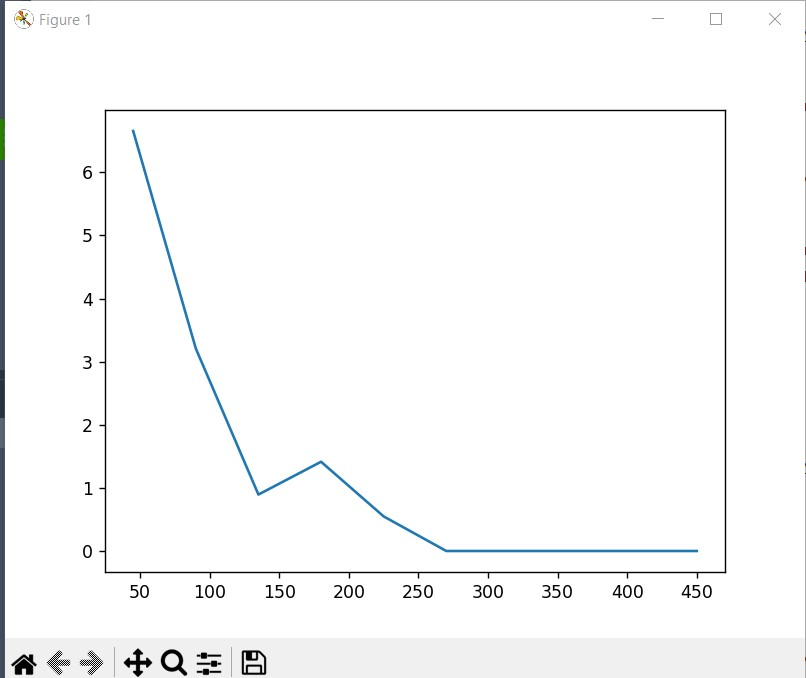
\includegraphics[width=0.75\textwidth]{perceptron_std.jpg}}
    \\\\
    

   
\end{homeworkProblem}

\pagebreak

%Part 3%
\begin{homeworkProblem}
    \textbf{\large MIRA}\\\\
    Same as the previous two cases. We plot faces. The plots are: time vs samples, mean vs samples, and std vs samples.
    \\\\
    {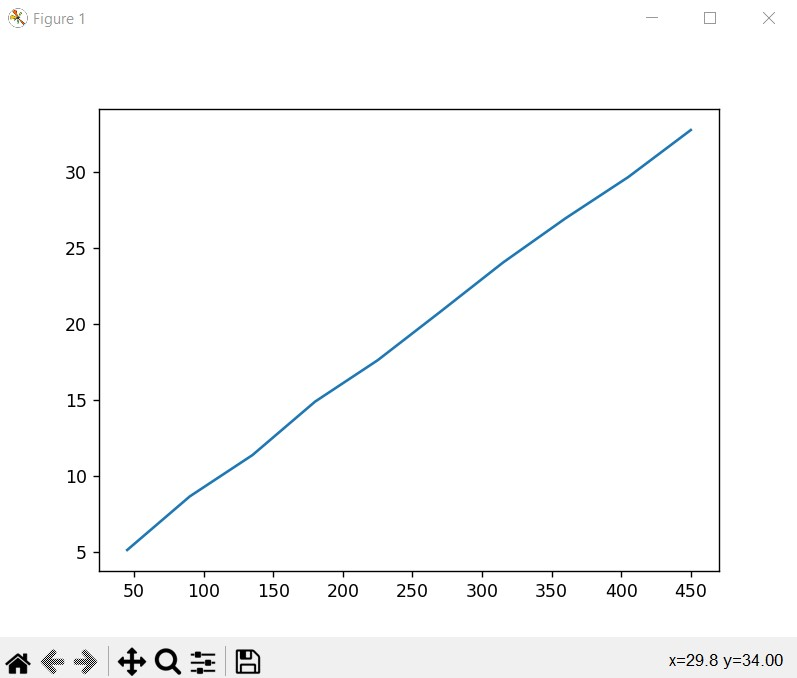
\includegraphics[width=0.75\textwidth]{mira_time.jpg}}
    \\\\
    {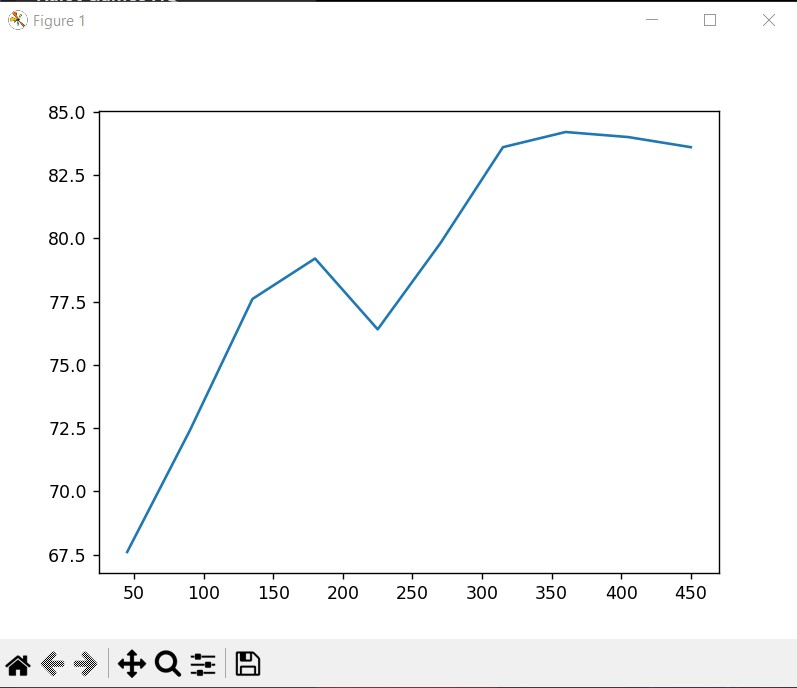
\includegraphics[width=0.75\textwidth]{mira_means.jpg}}
    \\\\
    {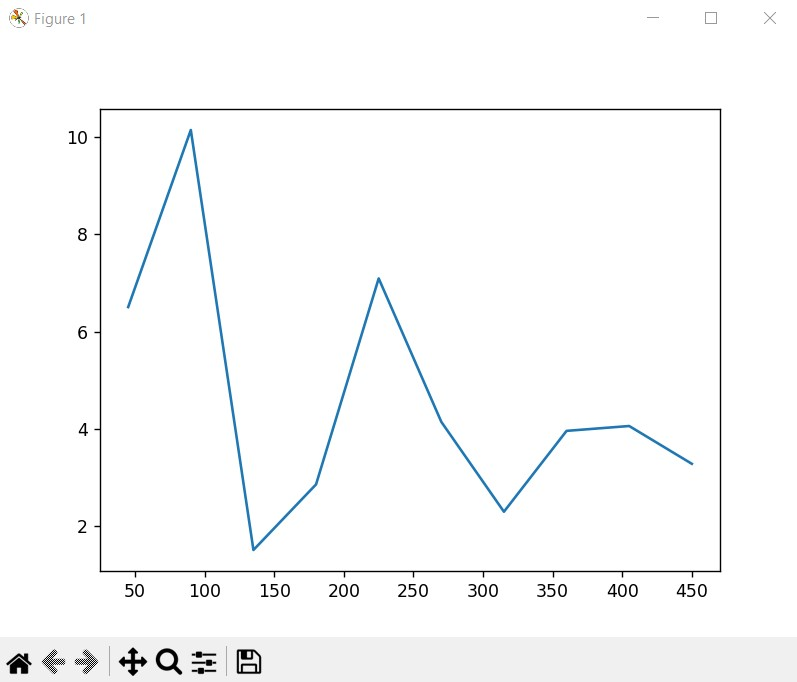
\includegraphics[width=0.75\textwidth]{mira_std.jpg}}
    \\\\
\end{homeworkProblem}

\pagebreak

%Part 4
\begin{homeworkProblem}
    \textbf{\large Comparative Analysis}\\\\
    
    For the full sample size, the average time for Naive Bayes was 13 seconds, the average time for perceptron was 7 seconds, and the average time for MIRA was 30 seconds. Our test set for all cases was 100 samples to construct these plots.
    The average accuracy for Naive bayes was 88 percent, the average accuracy for the perceptron was also 88 percent, and the average accuracy for MIRA was 85 percent. All standard deviations generally converge to zero, although MIRA has a slightly higher standard deviation of 2. In general, the first two algorithms perform quite well, and perceptron is the fastest and most accurate. The increased complexity of MIRA made it cost extra time. The learned lessons is that basic features, even raw pixel mapping, can be very effective and lead to quite good estimations, and of course that a greater size training set generally leads to best results. We also note that smoothing is quite effective in the Naive Bayes estimation and helps to prevent taking the logarithm of 0 in case a feature was 0.
    \\\\
\end{homeworkProblem}

\pagebreak

\end{document}